\tolerance=10000
\documentclass[conference]{IEEEtran}
\usepackage{xcolor}
\usepackage{mathtools}
\usepackage{enumerate}
\usepackage{multirow}
\usepackage{hyperref}
\usepackage{amssymb}
\usepackage{amsmath}
\usepackage{eqnarray}
\usepackage{booktabs}
\usepackage{array}
\usepackage[]{algorithm}
\usepackage{clrscode3e}
\usepackage[pdftex]{graphicx}

%\usepackage{etoolbox}
%\AtBeginEnvironment{algorithmic}{\small}
%\usepackage{subfig}
% tricks for saving space
\usepackage[font={small}]{caption,subfig}  % small fonts in captions
\setlength{\abovecaptionskip}{1ex}
\setlength{\belowcaptionskip}{1ex}
\setlength{\floatsep}{1ex}
\setlength{\textfloatsep}{1ex}

\DeclarePairedDelimiter{\ceil}{\lceil}{\rceil}
\DeclarePairedDelimiter{\floor}{\lfloor}{\rfloor}
\DeclarePairedDelimiter{\angled}{\langle}{\rangle}

\begin{document}

%%%%%%%%%%%%%%%%%%%%%%%%%%%%%%%%%%%%%%%%%%%%%%%%%%%%%%%%%%%%%%%%%%%%%%%
%%%%%%%%%%%%%%%%%%%%%%%%%%%%%%%%%%%%%%%%%%%%%%%%%%%%%%%%%%%%%%%%%%%%%%%
%%
%% TITLE
%%
%%%%%%%%%%%%%%%%%%%%%%%%%%%%%%%%%%%%%%%%%%%%%%%%%%%%%%%%%%%%%%%%%%%%%%%
%%%%%%%%%%%%%%%%%%%%%%%%%%%%%%%%%%%%%%%%%%%%%%%%%%%%%%%%%%%%%%%%%%%%%%%

\title{ZNN\emph{i} -- Maximizing the Inference Throughput of 3D
  Convolutional Networks on Multi-Core Machines and GPUs}

\author{\IEEEauthorblockN{Aleksandar Zlateski\IEEEauthorrefmark{1},
    Kisuk Lee\IEEEauthorrefmark{2}}
  \IEEEauthorblockA{\IEEEauthorrefmark{1}Electrical Engineering and
    Computer Science Dept.\\ \IEEEauthorrefmark{2}Brain and
    Cognitive Sciences Dept.\\ Massachusetts Institute of
    Technology\\ Cambridge, MA 02139 USA\\ \IEEEauthorrefmark{1}{\tt
      zlateski@mit.edu}, \IEEEauthorrefmark{2}{\tt kisuklee@mit.edu}}
  \and \IEEEauthorblockN{H. Sebastian Seung}
  \IEEEauthorblockA{Princeton Neuroscience Institute\\ and Computer
    Science Dept.\\ Princeton University\\ Princeton, NJ 08540
    USA\\ {\tt sseung@princeton.edu} }}


\maketitle
%\thispagestyle{empty}

%%%%%%%%%%%%%%%%%%%%%%%%%%%%%%%%%%%%%%%%%%%%%%%%%%%%%%%%%%%%%%%%%%%%%%%
%%%%%%%%%%%%%%%%%%%%%%%%%%%%%%%%%%%%%%%%%%%%%%%%%%%%%%%%%%%%%%%%%%%%%%%
%%
%% ABSTRACT
%%
%%%%%%%%%%%%%%%%%%%%%%%%%%%%%%%%%%%%%%%%%%%%%%%%%%%%%%%%%%%%%%%%%%%%%%%
%%%%%%%%%%%%%%%%%%%%%%%%%%%%%%%%%%%%%%%%%%%%%%%%%%%%%%%%%%%%%%%%%%%%%%%


\begin{abstract}

We present a novel parallel algorithm for 3D ConvNet inference on
multi-core shared memory machines.  We also present a novel algorithm
for ConvNet inference on the GPU that uses less memory.  We also
present an algorithm that uses the GPU and host ram to improve the
throughput.  As well as CPU-GPU combined algorithm.

We compare discuss the advantages and disadvantages of all approaches.

We compare our algorithms to publicly available implementation (on the
same hardware) and observe great speedup.

\end{abstract}

%%%%%%%%%%%%%%%%%%%%%%%%%%%%%%%%%%%%%%%%%%%%%%%%%%%%%%%%%%%%%%%%%%%%%%%
%%%%%%%%%%%%%%%%%%%%%%%%%%%%%%%%%%%%%%%%%%%%%%%%%%%%%%%%%%%%%%%%%%%%%%%
%%
%% INTRODUCTION
%%
%%%%%%%%%%%%%%%%%%%%%%%%%%%%%%%%%%%%%%%%%%%%%%%%%%%%%%%%%%%%%%%%%%%%%%%
%%%%%%%%%%%%%%%%%%%%%%%%%%%%%%%%%%%%%%%%%%%%%%%%%%%%%%%%%%%%%%%%%%%%%%%

\section{Introduction}

cuDNN is described here~\cite{chetlur2014cudnn}

We do max fragment pooling as described here~\cite{giusti2013fast}.
Except that we are limiting the sizes of our output patches to have
each dimension equal to the cartesian product of all corresponding
dimensions of all pooling windows in the network.

We care about throughput -- not latency in this case.  This is because
we assume that we need to do inference on a large amount of data.

Hence, self-tuning time and latency are negligible.  Self-tuning
because it only has to be done once; latency because the data is huge.
Examples -- videos, EM data, tons of images (FB?).

Relate to ZNN for training as training has to be optimized for
latency.

\section{Max fragment pooling}

We should not use batches (except sometimes)

\begin{figure}
  \centering
  \subfloat[]{\protect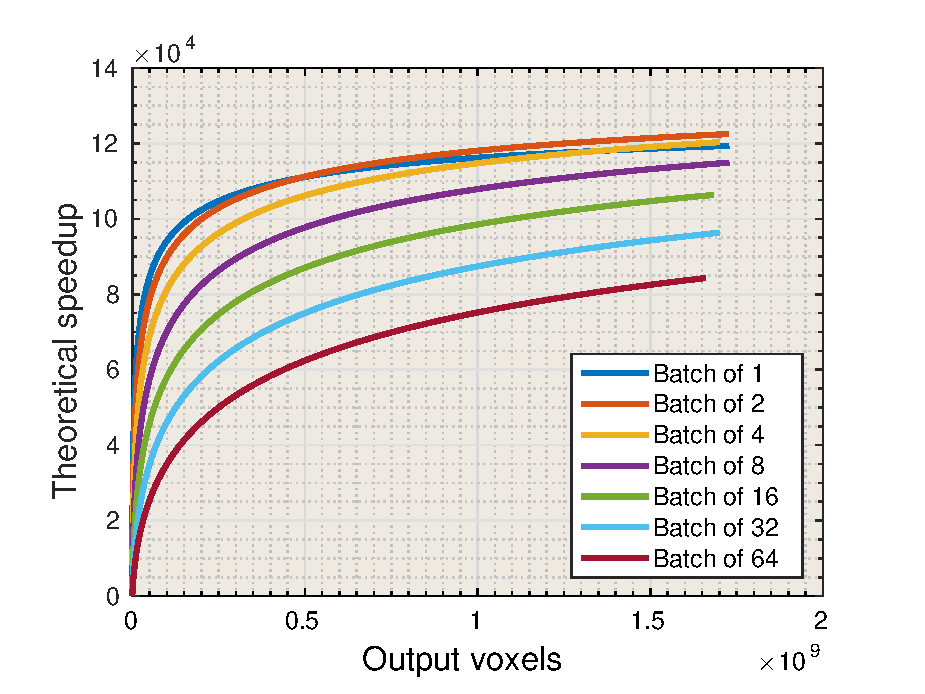
\includegraphics[width=0.24\textwidth]
    {fig/fft_batch_speedup.eps}}
  \subfloat[]{\protect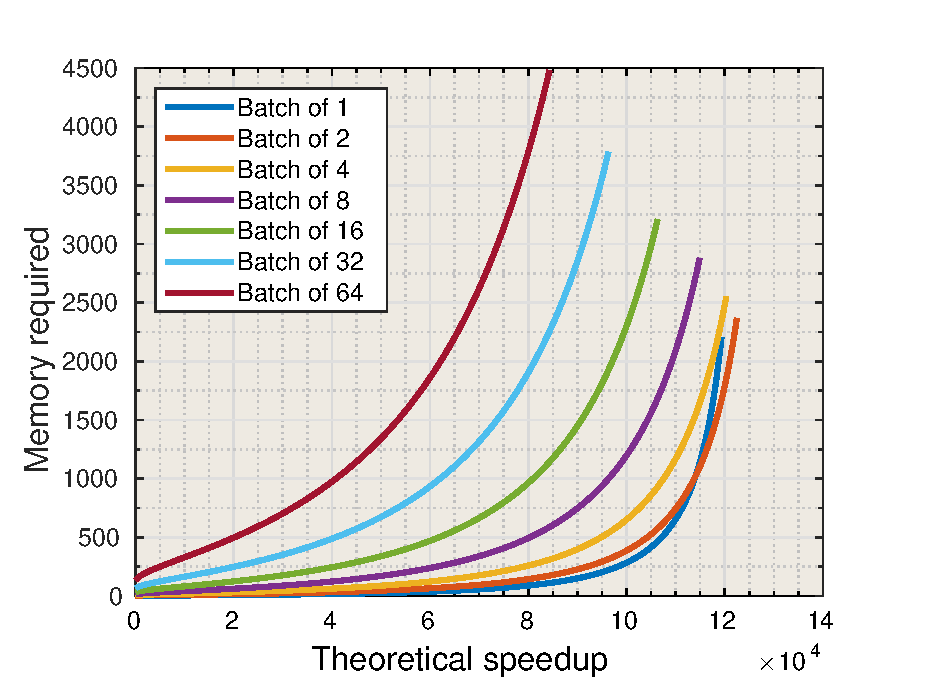
\includegraphics[width=0.24\textwidth]
    {fig/fft_mem_speedup.eps}}

  \caption{Explains why we should not use batches ever!}
  \label{fig:batch_explanation}
\end{figure}



We reduce the number of operations per output sample by:
\begin{enumerate}
\item Using max fragment pooling.
\item Choosing optimal size for the output image as well as the batch
  size.
\item Using \emph{pruned FFTs} for computing the FFTs of the kernels
  and images.
\end{enumerate}

We improve the throughput by parallelizing the algorithm over multiple
available cores, while using little memory overhead per running
thread.


\section{Padded pruned FFT}

A 3D FFT transform is obtained by computing 1D FFTs along the three
dimensions.  When computing a transform of a padded 3D image, many of
these 1D transforms will operate on all $0$ elements.  These
transforms are unnecessary as FFT of a zero vector is a zero vector.

A convolution of a 3D image with a kernel is obtained by first zero
padding the image and the kernel to the same size, after which we
perform the transform of both the padded image and kernel.  The
inverse transform of the point-wise product of the two transforms will
contain the result of the convolution.

We can reduce the amount of computation by computing only necessary 1D
transforms.  For instance, when computing the FFT of trainable kernel
of size $k^3$ zero padded to size of $n^3$, instead of naively
computing $n^2$ 1D FFTs each dimension, which takes $C n^3 \log n^3$
we could first only do $k^2$ FFTs along one direction, then $k \times
x$ along then next, and finally $n^2$ along the last direction.  This
way we reduce the computational cost from $C n^3 \log n^3$ to $C n\log
n[k^2 + k \cdot n + n^2]$.  As most of the FFTs are performed on
kernels, when $k << n$, we could reduce the computation cost by almost
two thirds.


\begin{figure}
  \begin{center}
  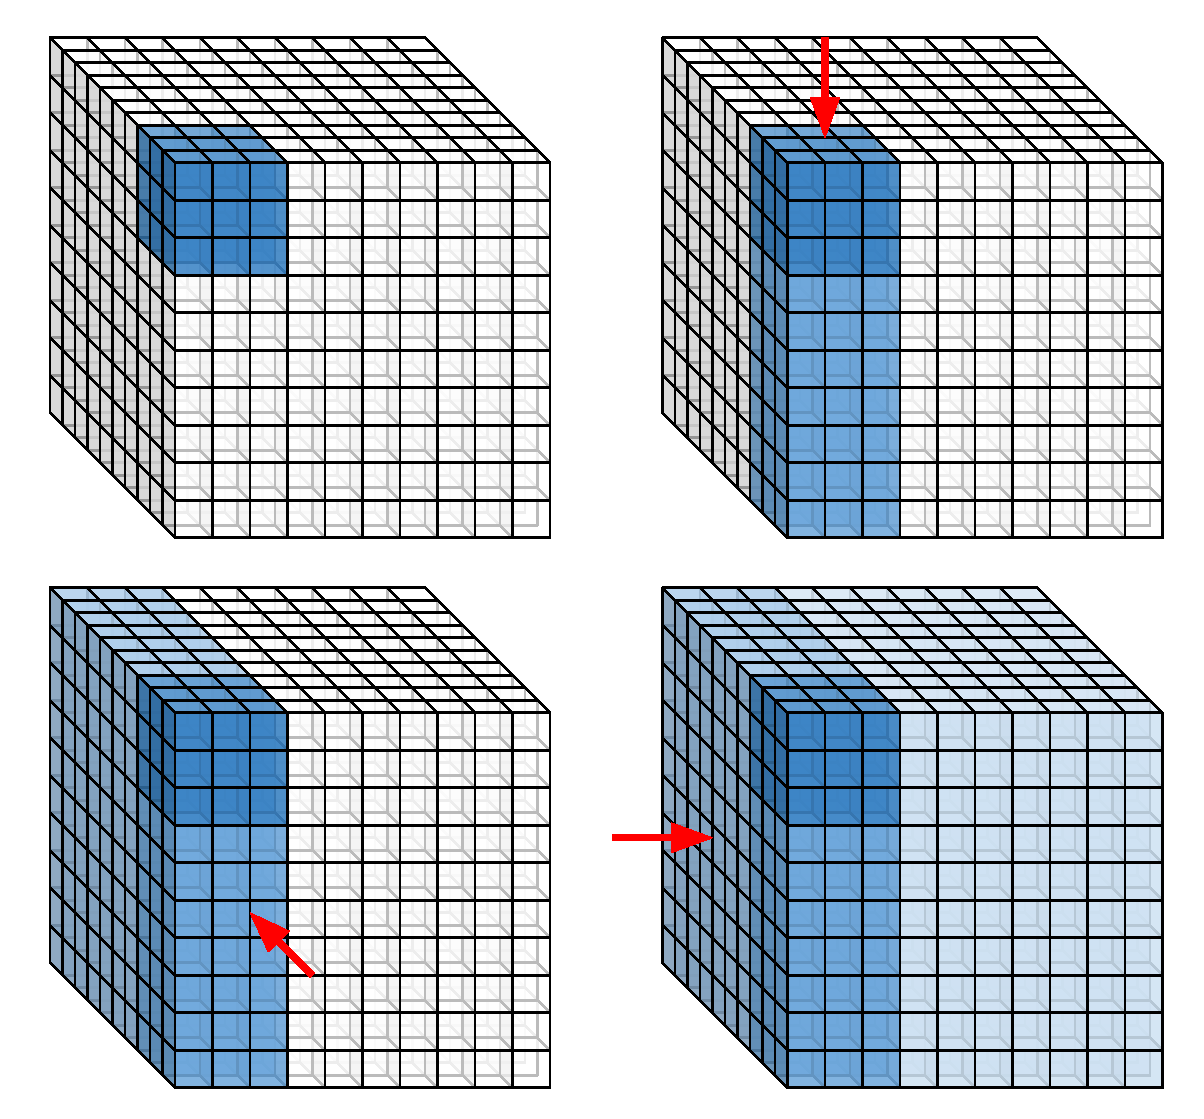
\includegraphics[width=0.65\columnwidth]{fig/pruned_ffts.pdf}
  \end{center}
  \caption{Pruned FFTs.}
  \label{fig:pruned_ffts}
\end{figure}

\subsection{FFT based convolution}

The convolution theorem states that the fourier transform of a
convolution euqals the pointwise product of the fureier transforms of
the signals.  In the descrete case, the theorem is given by:

$$x \ast y = DTFT^{-1}[DTFT\{x\} \cdot DTFT\{y\}]$$

When implementing the FFT based convolution, the signals $x$ and $y$
are first zero-padded to the same size.  The inverse FFT of the
point-wise product contains the result of the convolution.  The
signals $x$ and $y$ can be zero-padded to any size, as long as their
size is equal.  We zero-pad the signals to sizes for which we have
very efficient FFT algorithms.  On the CPU we either use sizes that
can be written in the form of $2^a3^b5^c7^d11^e13^f$.  When Intel MKL
is used any such size is allowed, however, when fftw is used we only
allow sizes for which $e+f$ is either $0$ or
$1$~\cite{frigo1999fftw,frigo1998fftw}.  On the GPU we use
cuFFT~\cite{nvidia2010cufft}, which has optimized algorithms only for
sizes of the form $2^a3^b5^c7^d$.

The main functionality required by our algorithms is performing FFT
(and inverse FFT) of an image of size $x \times y \times z$
zero-padded to the size of $x' \times y' \times z'$.

\subsection{CPU implementation}

We present both a serial and parallel algorithm for performing a FFT
transform of a single 3D image.

First, the image of size $x \times y \times z$ is zero padded to the
size $x' \times y \times z$.  Note that this can be easily implemented
by doing a linear copy of the memory, and zero padding the rest.

We then perform $y \cdot z$ 1D real to complex FFTs along $x$
direction.  The transform is performed out of place into a
pre-allocated, and zero initialized complex 3D image of size
$\floor{\frac{x'}{2}} + 1 \times y' \times z'$.

After that we perform in-place 1D transforms along $y$ and finally
along $z$.  The difference between the serial and the parallel
algorithm is only in the way we are performing the 1D transforms -
either in serial, or by $N$ workers in parallel (can be thought of as
parallel for).

The memory overhead of the transform is due to the fact that we have
to store the padded $x' \times y \times z$ array before the first real
to complex FFT.

The inverse FFT can be computed in exact same way, just taking the
steps in reverse order.

\subsection{GPU implementation}

On the GPU, we always perform a batch of size $b$ of 3D FFTs.  This is
due to the fact that the GPUs have more effective threads and we want
to saturate the computational power of the GPU.

A set of $b$ 3D images can be represented as a 4D tensor.  We need to
perform 1D FFTs along the three least significant dimensions.  The 3D
FFT is computed by series of tensor transforms~\footnote{This is known
as a \texttt{permute} function in MATLAB} and 1D FFTs along the least
significant dimension of the permuted tensor.

Assume that we want to compute the FFT transforms of $b$ 3D images
each of size $x \times y \times z$ padded to $x' \times y' \times z'$.
The input is therefore a 4D tensor $I$ of dimensions $b \times
x \times y \times z$.

We first perform in--place real to complex 1D transforms along the $z$
direction. We prepare the input by extending the 4D tensor along the
$z$ direction to fit the result.  The transform will need to contain
$z'' = z' / 2 + 1$ complex numbers, and we need twice as many reals.
A 4D tensor $I^1$ of size $b \times x \times y \times 2z'')$ is first
initialized to zero, and appropriate elements from the input are
filled in (elements $I_{i,j,k,l}$ get mapped to $I^1_{i,j,k,l}$ while
the rest of elements of $I^1$ are set to zero).

After which a batch of $b$ in--place real to complex 1D transforms are
performed.  The result represents a 4D complex tensor
$\widetilde{I}^1$ of size $b \times x \times y \times z''$.  Note that
all the 1D transforms are done on contiguous memory chunks (along the
least significant dimension).

In the next step we perform in-place complex to complex transforms
along the $y$ direction.  To do this the elements of $\widetilde{I}^1$
are permuted into another 4D tensor $\widetilde{I}^2$ of size
$b \times x \times z'' \times y'$, such that the element
$\widetilde{I}^1_{i,j,k,l}$ gets mapped to $\widetilde{I}^2_{i,j,l,k}$
and the rest of $\widetilde{I}^2$ is zero filled.  We then perform
in-place complex to complex transforms along the least significant
dimension of $\widetilde{I}^2$.

In the final step, we perform the transform along the $x$ direction.
We permute $\widetilde{I}^2$ into a new 4D complex tensor
$\widetilde{I}^3$ of size $b \times z'' \times y' \times x'$.  An
element $\widetilde{I}^2_{i,j,k,l}$ is mapped to
$\widetilde{I}^3_{i,k,l,j}$.  Finally once more complex to complex
in-place transforms are performed along the least significant
dimension of $\widetilde{I}^3$.

As we only perform point-wise multiplications of transformed images,
or take the inverse transforms of them we can just keep the result in
this representation -- not waste computation doing extra permuting.

The inverse transform can be performed taking the same steps in
reverse order.

{\bf Implementation details} 4D tensor permuting requires a lot of
index to index calculation, which can involve a lot expensive division
and modulus operations.  Sometimes these operations are more expensive
than the actual 1D FFT transforms performed.  We improve the
performances by only using multiplications by a pre--computed magic
numbers and shift operations as described in ~\cite{warren2013hacker}.
Image reshaping is easily implemented using the Thrust CUDA
library~\cite{bell2011thrust}.

We limit the large cuFFT memory overhead for computing batches of 1D
transforms by splitting the batch computation into sub--batches of 1D
transforms.  We make sure that the sub--batch size is still large
enough to utilize all the computational power, but limit the size so
that we limit the memory overhead.  (Maybe mention that we have to
keep the pointers to texture alignment?)

The memory overhead of the algorithm is due to the fact that we do
out-of-place permuting of the 4D tensor and requires space for
$b \cdot x \cdot y' \cdot z''$ complex numbers.  This is, however,
will not increase the memory overhead of our algorithm for
convolutional layer on the GPU already needs a temporary tensor of
size $b \cdot x' \cdot y' \cdot z''$ which can be used as scratch
space for computing the FFT transforms.

Additional, relatively small, overhead comes from the memory required
by cuFFT to perform a batch of 1D transforms.  By dividing the batch
into sub--batches we essentially limit this overhead to a pre--defined
constant amount of memory.

\section{Convolutional layers}

  Consider a convolutional layer with $f$ input feature--maps and $f'$
  output feature--maps.  The input to the layer is a set of $f$ 3D
  images, or a minibatch of size $S$ each having $f$ 3D input images.
  The $f$ images of each minimbatch are convolved with $f' \times f$
  3D kernels producing $f'$ output images.

  In the computational sense, the convolutional layer operates on two
  5D tensors.  The first 5D tensor $I$ represents all the 3D input
  images such that $I_{s,i}$ is the $i^{th}$ 3D image of the $s^{th}$
  minibatch.  The second 5D tensor $w$ represents the set of all
  convolution kernels.  The output of the layer can also be
  represented as a 5D tensor $O$, such that

  $$O_{s,j} = \sum_{1 \le i \le f} I_{s,i} \ast w_{j,i}$$
  for $1 \le s \le S$ and $1 \le j \le f'$.

  If the size of the input images is $\vec{n} = \angled{n_x, n_y,
  n_z}$ and the size of the kernels is $\vec{k}
  = \angled{k_x,k_y,k_z}$, then the inputs to a convolutional layer
  are a 5D tensor $I$ of size $S \times f \times n_x \times n_y \times
  n_z$ representing the images, and a 5D tensor $w$ of size $f' \times
  f \times k_x \times k_y \times k_z$ representing the kernels.  The
  output of the convolutional layer is another 5D tensor of size
  $S \times f' \times n_x' \times n_y' \times n_z'$, where $\vec{n}'
  = \vec{n} - \vec{k} + \vec{1}$.

\subsection{CPU algorithms}

  We propose three parallel algorithms for the convolutional layer
  that are suited for multi-core CPUs.  The first algorithm performs
  direct convolution, whereas the other two use FFT based
  convolutions.

\subsubsection{Direct convolution algorithm}

  \begin{algorithm}
    {\small
      \begin{codebox}
        \Procname{$\proc{Convolutional-Forward-FFT-CPU1}(I,w,b,f,f',\vec{n},\vec{k})$}
        \li $\vec{n}' = \vec{n} - \vec{k} + \vec{1}$
        \li $O \gets \proc{5D-Real-Tensor}(b,f',n'_x,n'_y,n'_z)$
        \li \kw{parallel for} $i \gets 0 \To b-1$
        \li   \Do \kw{parallel for} $j \gets 0 \To f'-1$
        \li     \Do \For $k \gets 0 \To f-1$
        \li     \Do $O_{i,j} \gets O_{i,j} + \proc{Convolve}(I_{i,k},w_{j,k})$
        \End \End \End
        \li $\proc{Free-Memory}(I)$
        \li \Return $O$
      \end{codebox}
    }

    \caption{Multi-core algorithm for a convolutional layer using direct
      convolution.}
    \label{alg:cpu_direct}
  \end{algorithm}

  The algorithm using direct convolution is showin in the
  Algorithm~\ref{alg:cpu_direct}.  The computation is parallelized by
  two $\kw{parallel for}$ loops such that each output image of each
  minimbatch is computed in parallel on a different working thread.
  The $\kw{parallel for}$ loops are implemented using intel$^{\small
    \textregistered}$ thread building blocks such that the work is
  evenly divided over the available cores.

  For the direct convolution we provide two implementations.  The
  first is a naive convolution implementation, and the second one is
  using Intel\^{}$\{$$\backslash$ textregistered$\}$ to perform
  convolutions.  MKL implementation is 2x faster on average, however
  it requires extra memory for a temporary image where a result of
  convolution is stored before accumulating it to the output image.
  When $c$ cores are available this yields a memory overhead of $c
  \times n_x' \times n_y' \times n_z'$.  The total amount of memory
  required for a layer is given in the
  Table~\ref{table:memory_requirements}.

  \begin{table}
    \centering
    \begin{tabular}{l >{$}l<{$}}
      \toprule
      CPU algorithm & \text{Memory required} \\
      \midrule
      Direct (naive) &
      S \cdot f \cdot n + S \cdot f' \cdot n'\\
      Direct (MKL) &
      S \cdot f \cdot n + S \cdot f' \cdot n' + T \cdot n' \\
      FFT algorithm 1 &
      \max
      \begin{cases}
        S \cdot f \cdot (n + \widetilde{n}) \\
        S \cdot f' \cdot n' + (S + 1) \cdot \widetilde{n}
      \end{cases} \\
      FFT algorithm 2 &
      \max
      \begin{cases}
        S \cdot f \cdot (n + \widetilde{n}) \\
        S \cdot (f + f') \cdot \widetilde{n} + T \cdot \widetilde{n} \\
        S \cdot f' \cdot (n' + \widetilde{n})
      \end{cases} \\
      \midrule
      GPU algorithm & \text{Memory required} \\
      \midrule
      cuDNN (default) &
      S \cdot f \cdot n + S \cdot f' \cdot n' \\
      cuDNN (precomp) &
      2S \cdot f \cdot n + S \cdot f' \cdot n' \\
      FFT &
      C + \max
      \begin{cases}
        S \cdot f \cdot (n + \widetilde{n}) + f \cdot \widetilde{n} \\
        S \cdot (f + f') \cdot \widetilde{n} + 2f \cdot \widetilde{n} \\
        S \cdot f' \cdot (n' + \widetilde{n}) + f' \cdot \widetilde{n}
      \end{cases} \\
      \bottomrule
    \end{tabular}

    \caption{Memory required by different implementations.}
    \label{table:memory_requirements}
  \end{table}

\subsubsection{FFT based algorithm 1}

  The first algorithm is very similar to the serial algorithm and is
  given in the algorithm listing~\ref{alg:cpu_fft_alg1}.  The
  computationally intensive operations in the algorithm are
  individually parallelized.  More specifically each FFT and inverse
  FFT transform is done in parallel as explained in the previous
  section.  The $\proc{Parallel-MAD}$ function computes a series of
  multiply-add operations in parallel by dividing the range into
  roughly equal sub-ranges, each of which is executed on a single
  core.

  \begin{algorithm}
    {\small
      \begin{codebox}
        \Procname{$\proc{Convolutional-Forward-FFT-CPU1}(I,w,b,f,f',\vec{n},\vec{k})$}
        \li $\vec{n}' = \vec{n} - \vec{k} + \vec{1}$
        \li $\vec{\widetilde{n}} = \proc{FFT-Optimal-Size}(\vec{n})$
        \li $\widetilde{I} \gets \proc{5D-Complex-Tensor}(b,f,\floor{\widetilde{n}_x/2}+1,\widetilde{n}_y,\widetilde{n}_z)$
        \li \For $i \gets 0 \To b-1$
        \li   \Do \For $j \gets 0 \To f-1$
        \li     \Do $\widetilde{I}_{i,j} \gets \proc{Parallel-FFT}(I_{i,j})$
        \End \End
        \li $\proc{Free-Memory}(I)$
        \li $O \gets \proc{5D-Real-Tensor}(b,f',n'_x,n'_y,n'_z)$
        \li $\widetilde{O} \gets \proc{4D-Complex-Tensor}(b,\floor{\widetilde{n}_x/2}+1,\widetilde{n}_y,\widetilde{n}_z)$
        \li $\widetilde{w} \gets \proc{3D-Complex-Tensor}(\floor{\widetilde{n}_x/2}+1,\widetilde{n}_y,\widetilde{n}_z)$
        \li \For $i \gets 0 \To f'-1$
        \li   \Do \For $j \gets 0 \To f-1$
        \li     \Do $\widetilde{w} = \proc{Parallel-FFT}(w_{i,j})$
        \li         \For $k \gets 0 \To b-1$
        \li           \Do $\proc{Parallel-MAD}(\widetilde{I}_{k,j}, \widetilde{w}, \widetilde{O}_{k})$
        \End \End
        \li   \For $k \gets 0 \To b-1$
        \li      \Do $O_{k,i} \gets \proc{Parallel-Inverse-FFT}(\widetilde{O}_{k})$
        \End \End
        \li $\proc{Free-Memory}(\widetilde{I})$
        \li $\proc{Free-Memory}(\widetilde{O})$
        \li $\proc{Free-Memory}(\widetilde{w})$
        \li \Return $O$
      \end{codebox}
    }

    \caption{Multi-core algorithm for a convolutional layer}
    \label{alg:cpu_fft_alg1}
  \end{algorithm}

  The memory requirement of the algorithm equals to the maximal amount
  of memory required by the algorithm at any single point of time
  during the execution.  Given in the table.



We propose two algorithms suited for multi-core CPUs.  The two
algorithms have different parallelization strategies and yield
different performance and memory usage.

Both algorithm consist of three stages.  In the first stage all the
transforms of the inputs are computed.  In the second stage FFTs of
the kernels are computed and point-wise products are accumulated.
Finally in the third stage the inverse transforms of the accumulated
products are computed obtaining the output images.

Breaking up the algorithm into three stages allows us to more
efficiently utilize the available memory.  After the first stage, the
memory used by the input images is not required, and can be freed.
After the second stage the memory used by the transforms of the input
images can also be freed.

\subsubsection{Direct convolution algorithm}


\subsubsection{FFT based algorithm 2}

\begin{figure}
  \begin{center}
  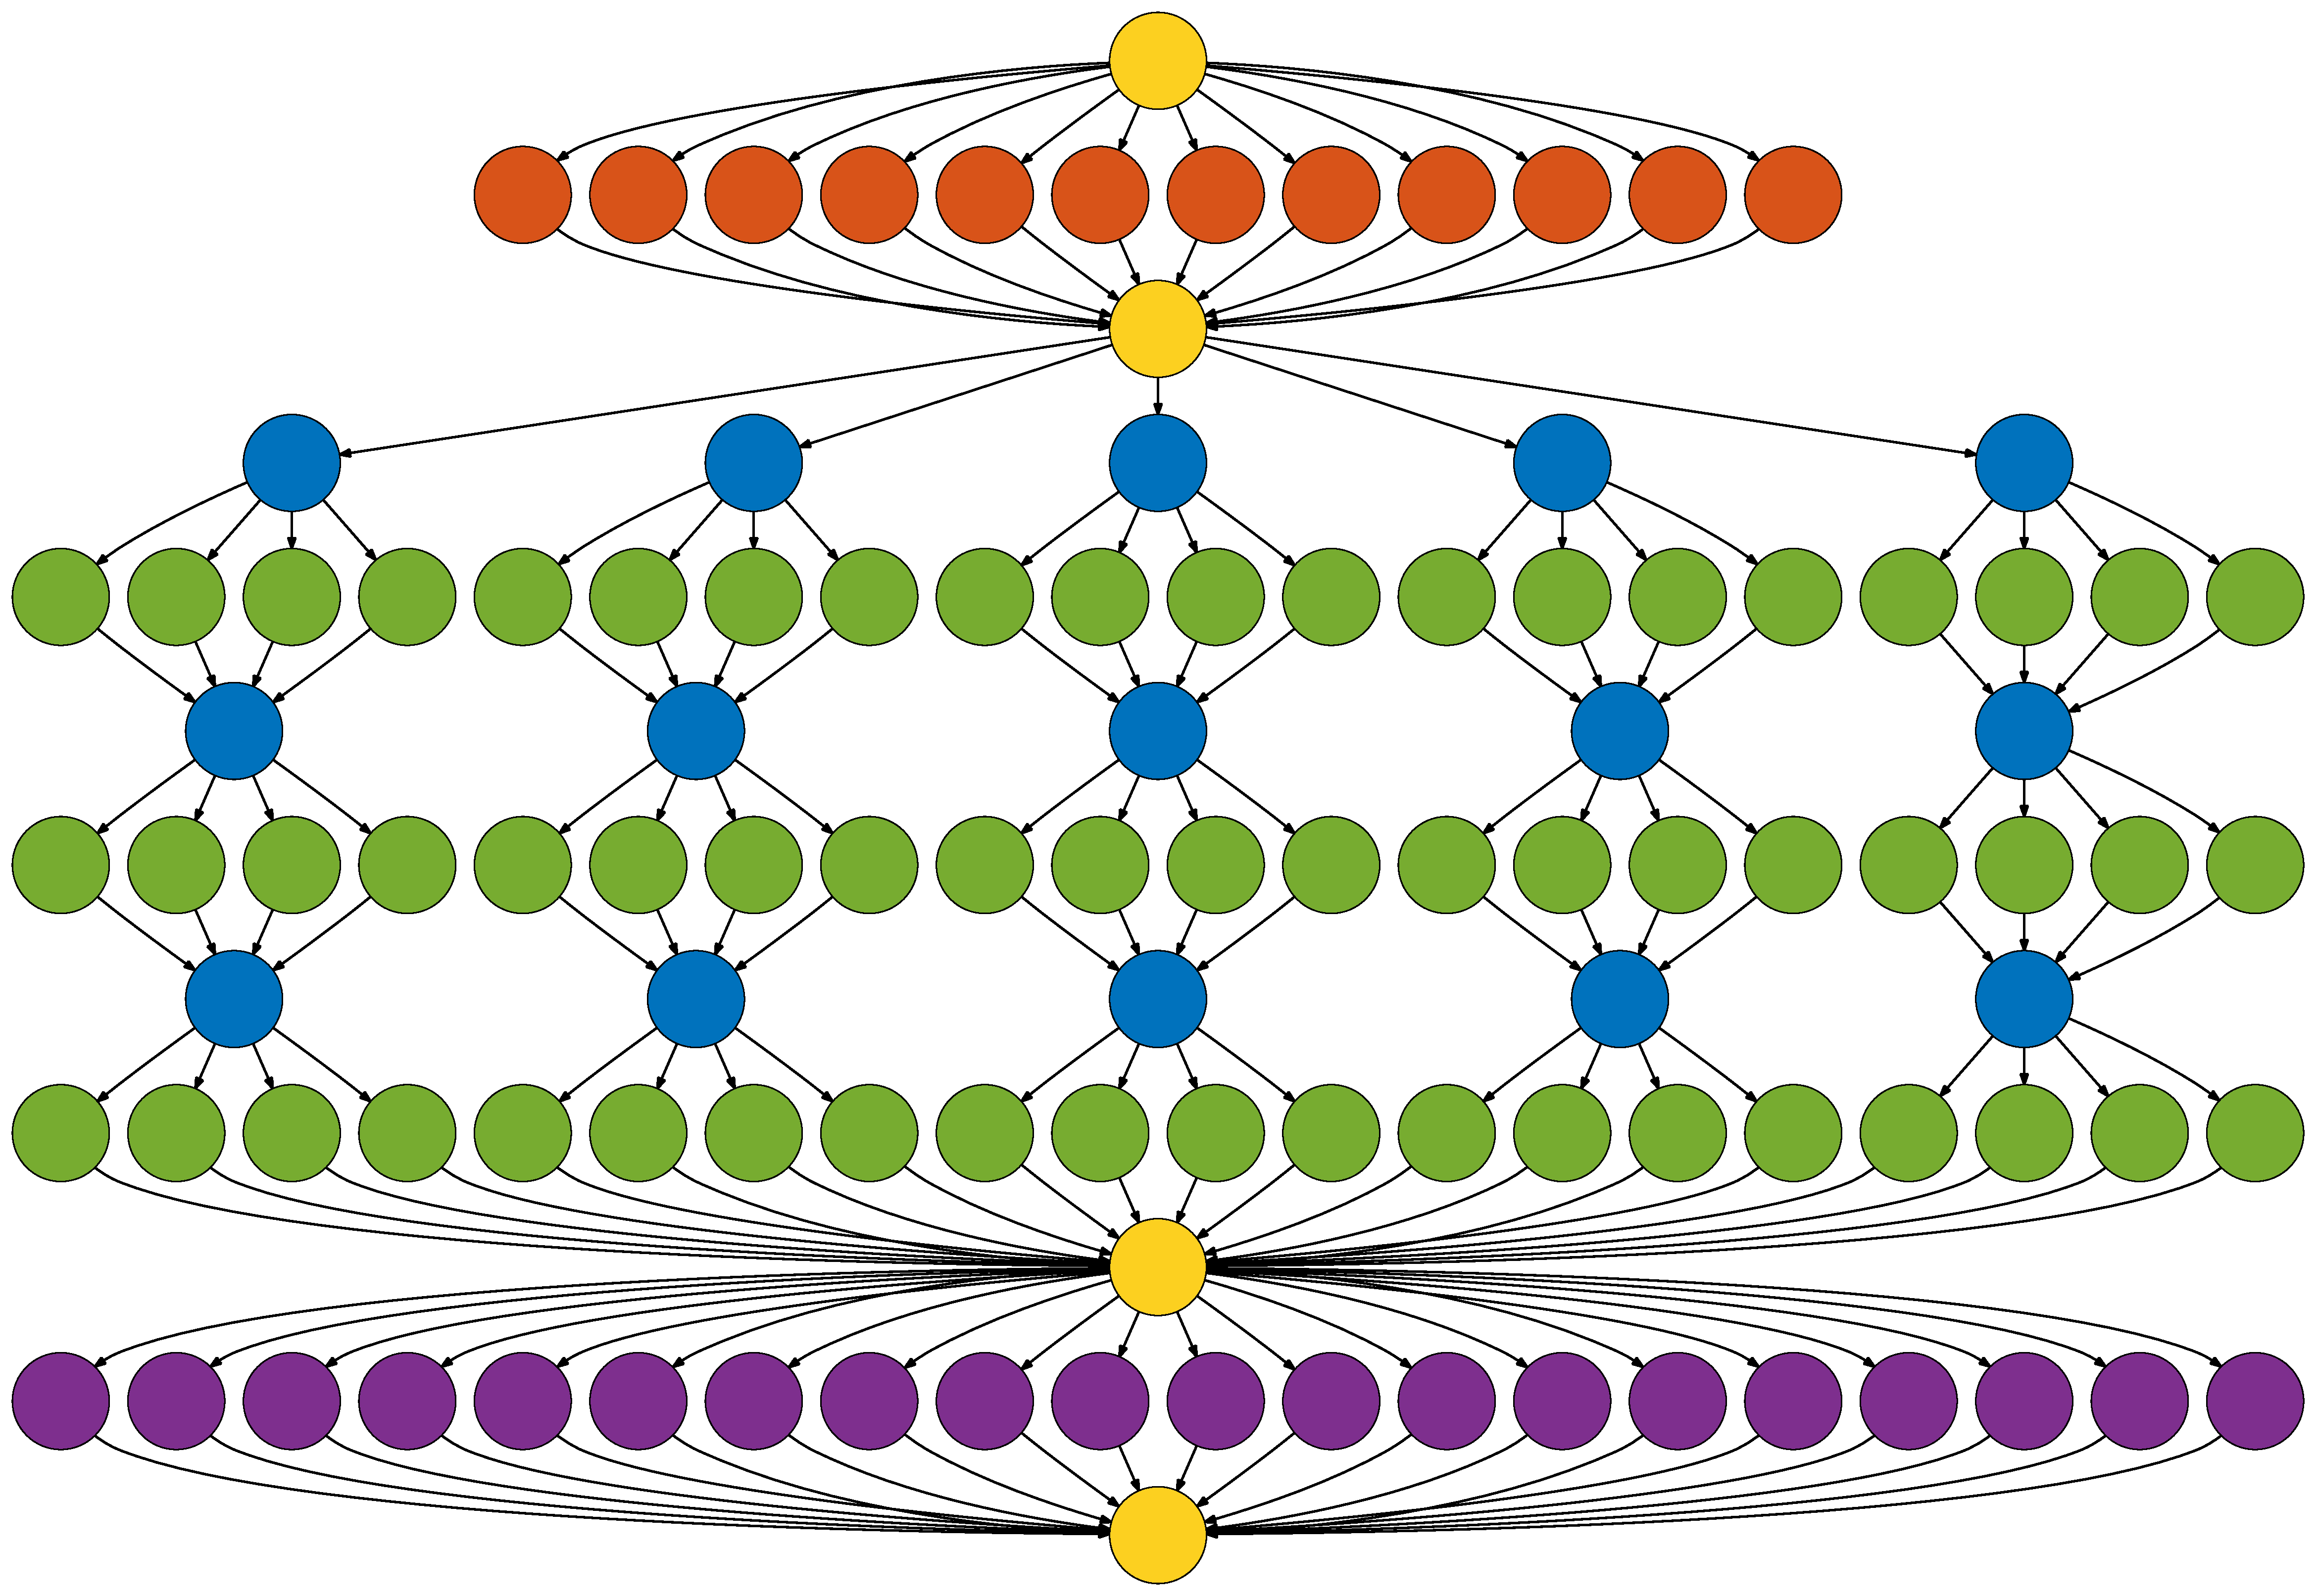
\includegraphics[width=0.95\columnwidth]{fig/deps}
  \end{center}
  \caption{Task dependencies of a convolutional layer.}
  \label{fig:task_deps}
\end{figure}


The main idea of the algorithm is to break up the computation of the
convolutional layer into tasks that operate on an independent chunk of
data.  We then create a task dependency graph and execute the tasks
using $N$ workers.  To increase cache locality the tasks are managed
using the work stealing scheduler, which means that each worker keeps
a list of local tasks as a stack (last task put on the stack will be
executed next)~\cite{reinders2007intel, willhalm2008putting}.  If a
local stack is empty, only then a worker \emph{steals} and executes a
task from other worker's queue.

We have 5 types of task, each of which performs relatively simple
work.  A task dependency diagram is shown on
figure~\ref{fig:task_deps}.

The first type of tasks (yellow) have two purposes.  They serve as
synchronization points, and they deal with memory management.  They
allocate memory required for the next stage and free the memory that
is not needed any more.  The topmost yellow task allocates memory for
the FFT transforms of all the input images, as well as working memory
for each of the $N$ workers.

The second task type (red) performs a transform of a single image of
the input.  Note that performing FFTs of image require some extra
working memory, which was allocated for each worker in the dependent
yellow task.  The number of such tasks will equal to the product of
the batch size and the number of input feature-maps.

After computing all the FFTs transforms of all the input images, we
can free the memory used by the images (as we don't need that
information anymore).  This is done by the second from the top yellow
task.  This yellow task also allocates memory for FFTs of all the
output images.

The next two task types are blue -- performs the FFT transform of a
kernel, and green -- multiplies the FFT transform of the kernel with
the appropriate FFT transform of the input image and adds to the
appropriate sum.  The task dependency is designed such that there's
never two workers trying to access the same memory.  Notice that the
blue tasks form some sort of a grid.  The blue tasks in each column
operate on the same output feature map, and blue tasks in each row
operate on the same input feature map.  More specifically a blue task
in column $i$ and row $j$ represents performing the FFT of the kernel
$k_{i,j}$.  For each blue task there is a number of green tasks equal
to the batch size.

\subsection{GPU implementations}

\subsubsection{Direct convolution using CuDNN}

\subsubsection{FFT based algorithm}


\begin{algorithm}
  {\small
  \begin{codebox}
    \Procname{$\proc{Convolutional-Forward-FFT-GPU}(I,w,b,f,f',x,y,z)$}
    \li $\widetilde{I} \gets \proc{5D-Complex-Tensor}(b,f,\floor{x/2}+1,y,z)$
    \li \For $i \gets 0 \To b-1$
    \li   \Do $\widetilde{I}_{i} \gets \proc{GPU-Parallel-FFT}(I_{i})$
    \End
    \li $\proc{Free-Memory}(I)$
    \li $\widetilde{O} \gets \proc{5D-Complex-Tensor}(b,f',\floor{x/2}+1,y,z)$
    \li \For $i \gets 0 \To f'-1$
    \li    \Do $\widetilde{w}_{i} = \proc{Parallel-FFT}(w_{i})$
    \li        \For $j \gets 0 \To b-1$
    \li           \Do $p \gets \proc{Parallel-Mult}(\widetilde{w}_{i}, \widetilde{I}_{j})$
    \li               $\widetilde{O}_{j,i} \gets \proc{Parallel-Accumulate}(p)$
    \End \End
    \li $\proc{Free-Memory}(\widetilde{I})$
    \li $O \gets \proc{5D-Real-Tensor}(b,f',x,y,z)$
    \li \For $i \gets 0 \To b-1$
    \li   \Do $O_{i} \gets \proc{GPU-Parallel-Inverse-FFT}(\widetilde{O}_{i})$
    \End
    \li $\proc{Free-Memory}(\widetilde{O})$
    \li \Return $O$
  \end{codebox}
  }

  \caption{FFT based convolutional layer algorithm for the GPU.}
  \label{alg:gpu_alg}
\end{algorithm}

\section{Algorithms for the max fragment pooling layers}



\subsection{CPU algorithm}
\subsection{GPU algorithm}

\section{Sliding window inference}

We describe how sliding window works.  Reference ZNN paper and other
papers.  Explain a bit about our implementation.

Also explain how sparse inference works, as we will use that on the
GPU -- only available implementation in 3D.

Explain how the FLOPs per output voxels are computed.

Figures -- chars of FLOPS vs Memory for different algorithms.

Note -- The tables in the previous section are correct even when
rarefied kernels are used, the only thing that changes is the size of
the output image that now equals $n' = n - (k-1)*r$, where $r$ is the
sparseness of the kernel.



\begin{figure}
  \begin{center}
  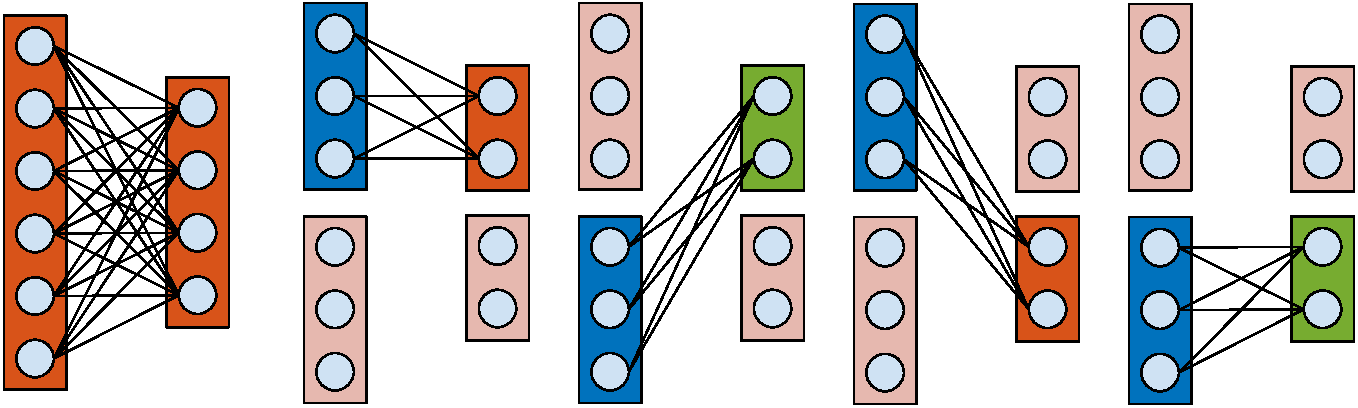
\includegraphics[width=0.95\columnwidth]{fig/gpuram.pdf}
  \end{center}
  \caption{Partial loading of data to the device.}
  \label{fig:partial_exec}
\end{figure}

Pooling layers use CUDNN.

Direct convolutional layers also use CUDNN.  If possible they use the
pre--computed gemm which requires workspace memory.  The cases when
this is possible is not well documented so we experimentally determine
whether we can use it.

\begin{figure*}
  \centering
  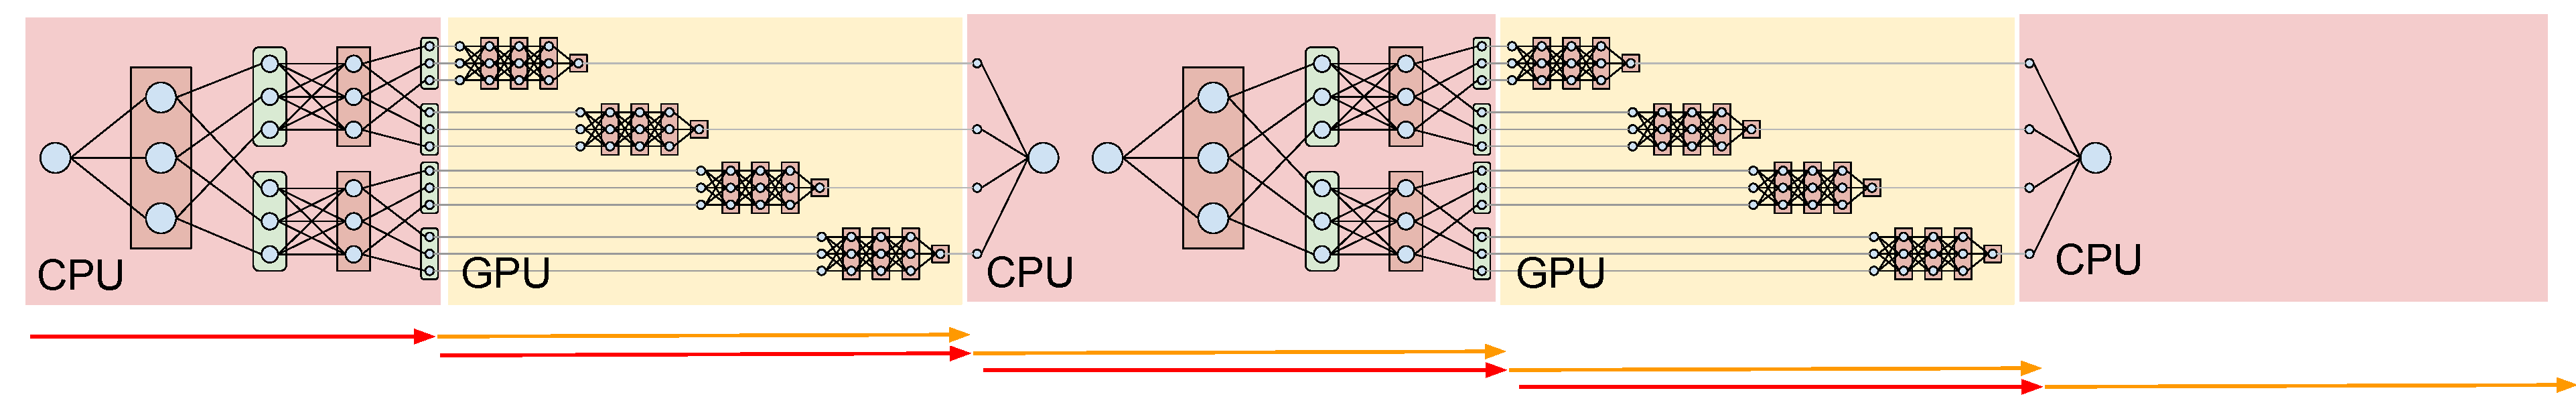
\includegraphics[width=0.9\textwidth]{fig/fusion.pdf}
  \caption{CPU--GPU combined approach}
  \label{fig:fusion}
\end{figure*}


FFT convolutional layers are implemented in the following way.  For
each layer we do the following.  We transform all the inputs first.
We break up the input into largest possible chunks that can be
transformed with CUFFTPLANN.  Once we have all the input transforms
(of all the images and bathes) we compute one output image at the
time.  For $i$-th output image we compute FFTs of all the relevant
kernels, then for each batch we compute the point-wise product of the
FFTs of the input images and the FFTs of the kernels.  We accumulate
the result into a single image using a matrix vector product CUBLAS
where the vector has all ones.  We repeat the process for every $i$-th
output of every batch, as we want to re-use the FFTs of the computed
kernels.

Finally we compute the inverse transform of the output images, scale
them appropriately, add the bias and apply the transfer function.

We carefully design the steps in order to minimize the extra memory
utilization.


\section{Experiments}

\subsection{Purely convolutional networks}
\subsection{Max-pooling convolutional networks}


\begin{figure*}[h!t]
  \centering
  \subfloat[]{\protect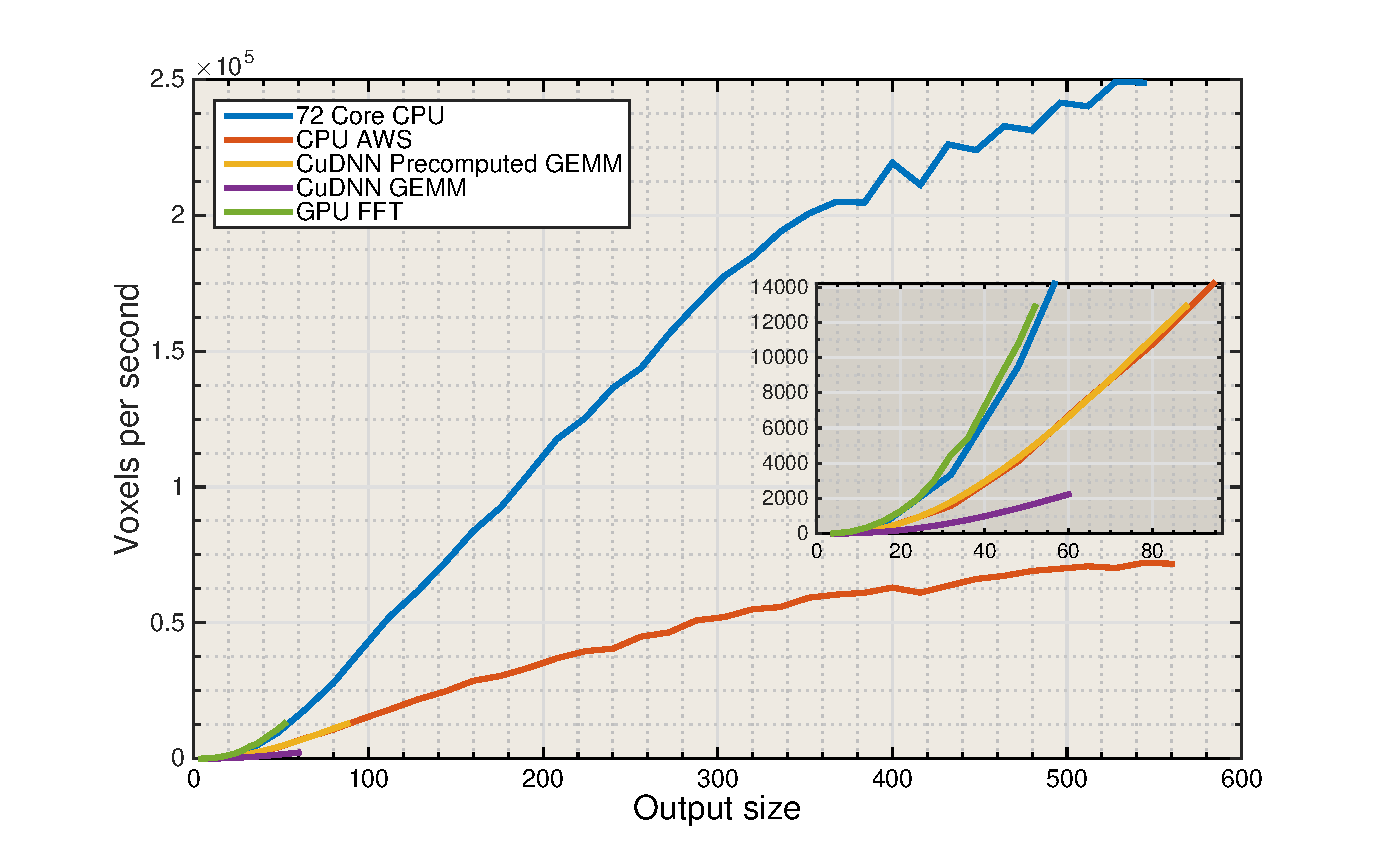
\includegraphics[width=0.44\textwidth]
    {fig/m96.eps}}
  \subfloat[]{\protect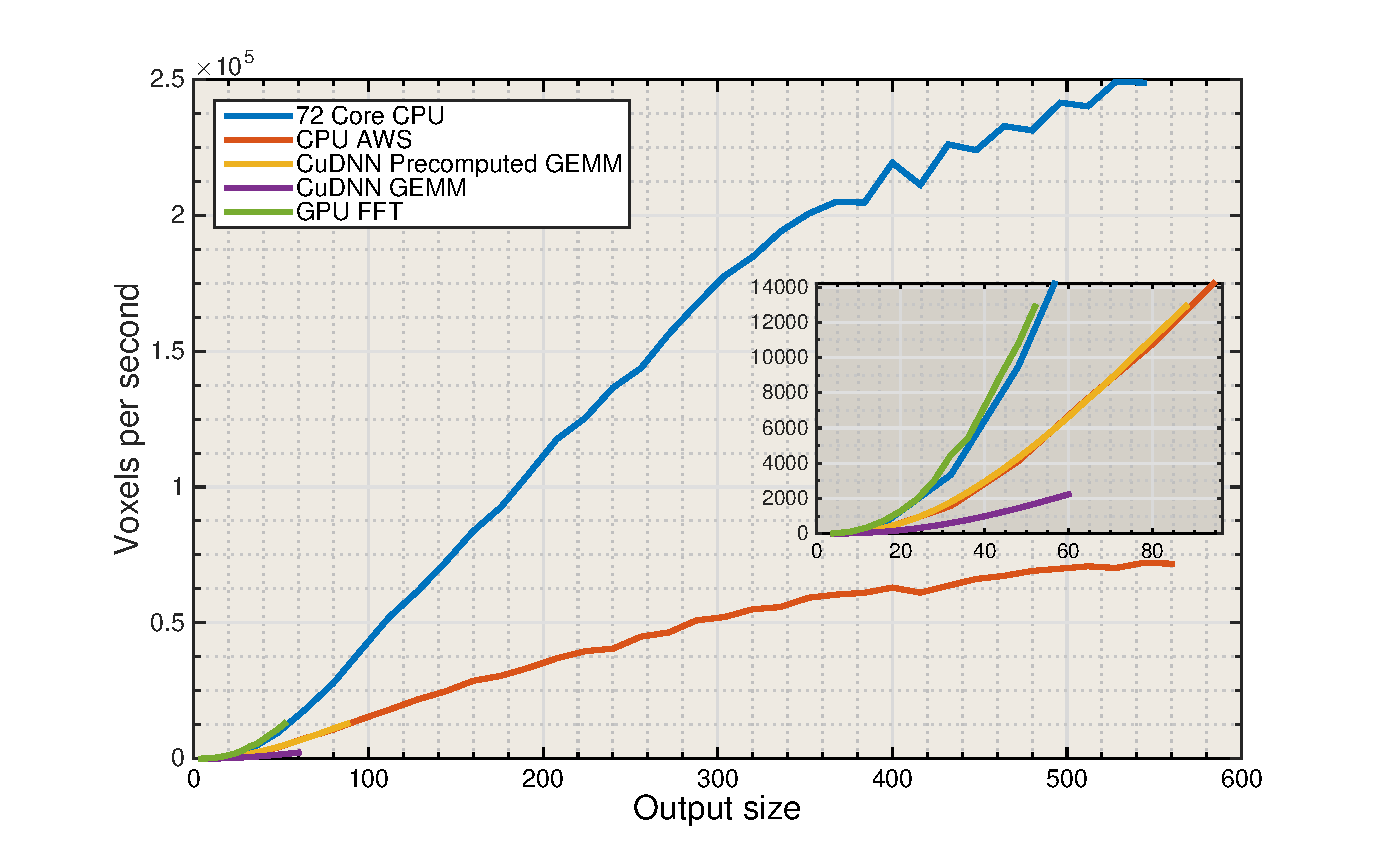
\includegraphics[width=0.44\textwidth]
    {fig/m96.eps}}
    \\
  \subfloat[]{\protect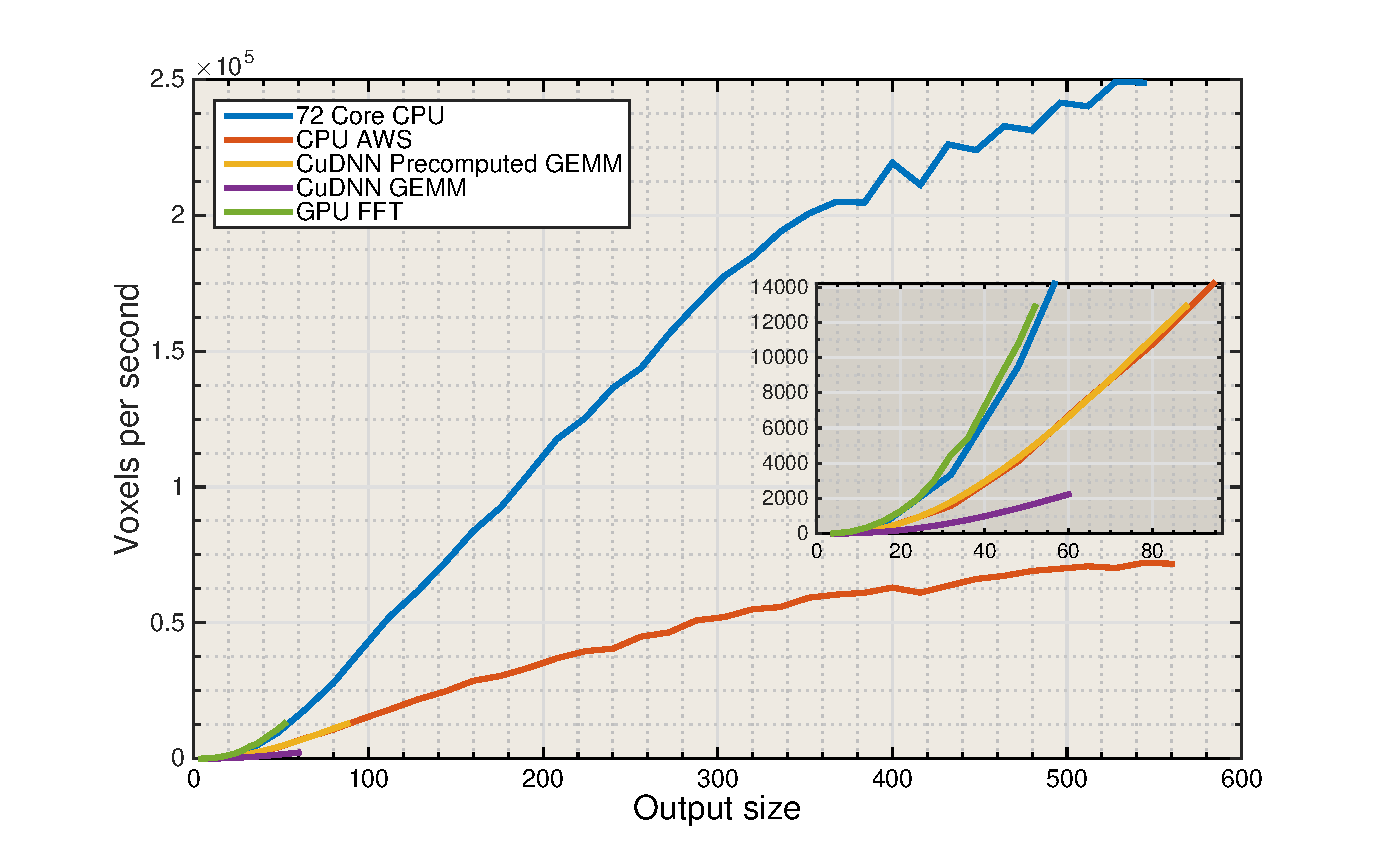
\includegraphics[width=0.44\textwidth]
    {fig/m96.eps}}
  \subfloat[]{\protect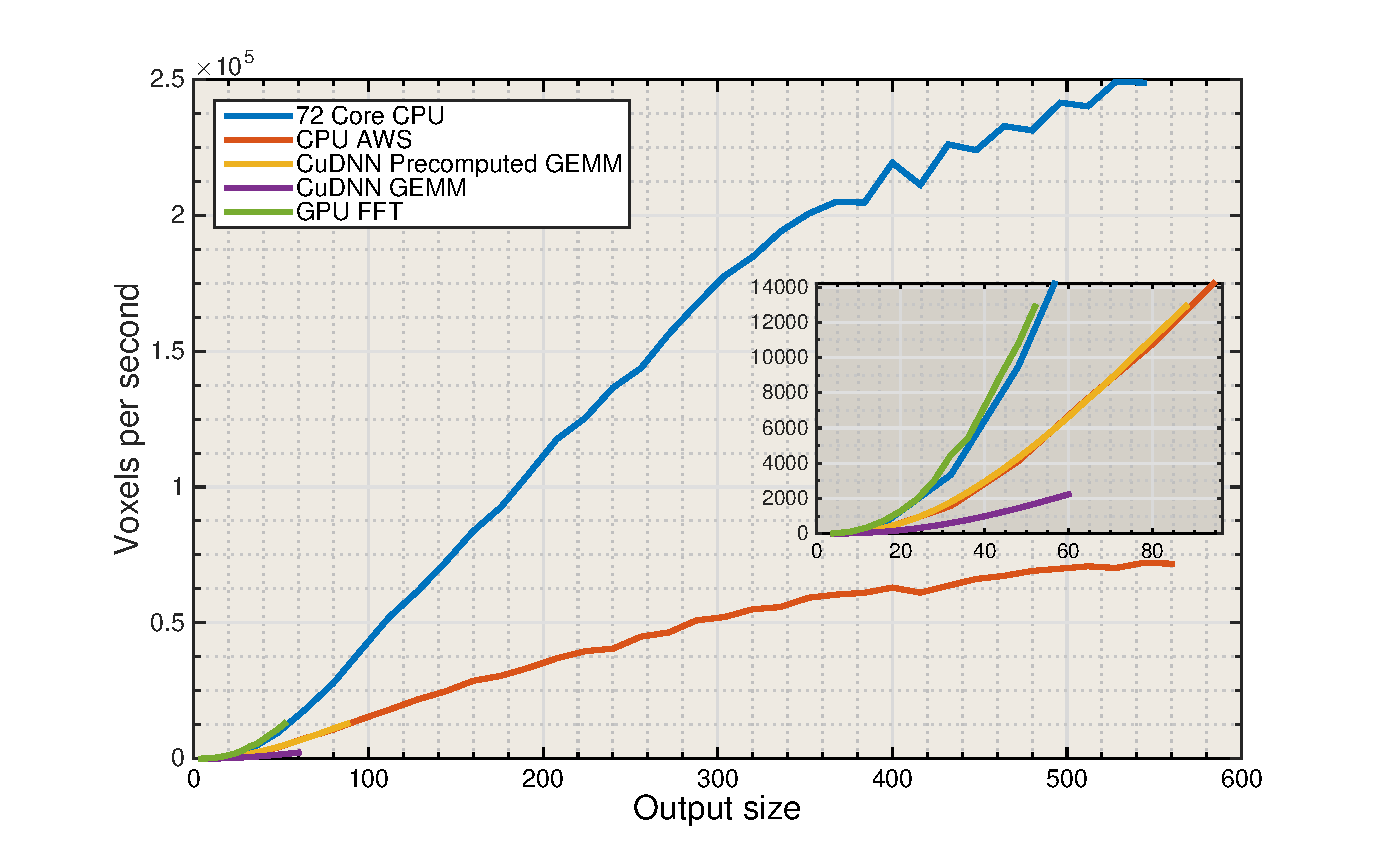
\includegraphics[width=0.44\textwidth]
    {fig/m96.eps}}

  \caption{Throughput vs output patch size for pooling networks
  }
  \label{fig:2dspeedups_threads}
\end{figure*}


\begin{figure*}[h!t]
  \centering
  \subfloat[]{\protect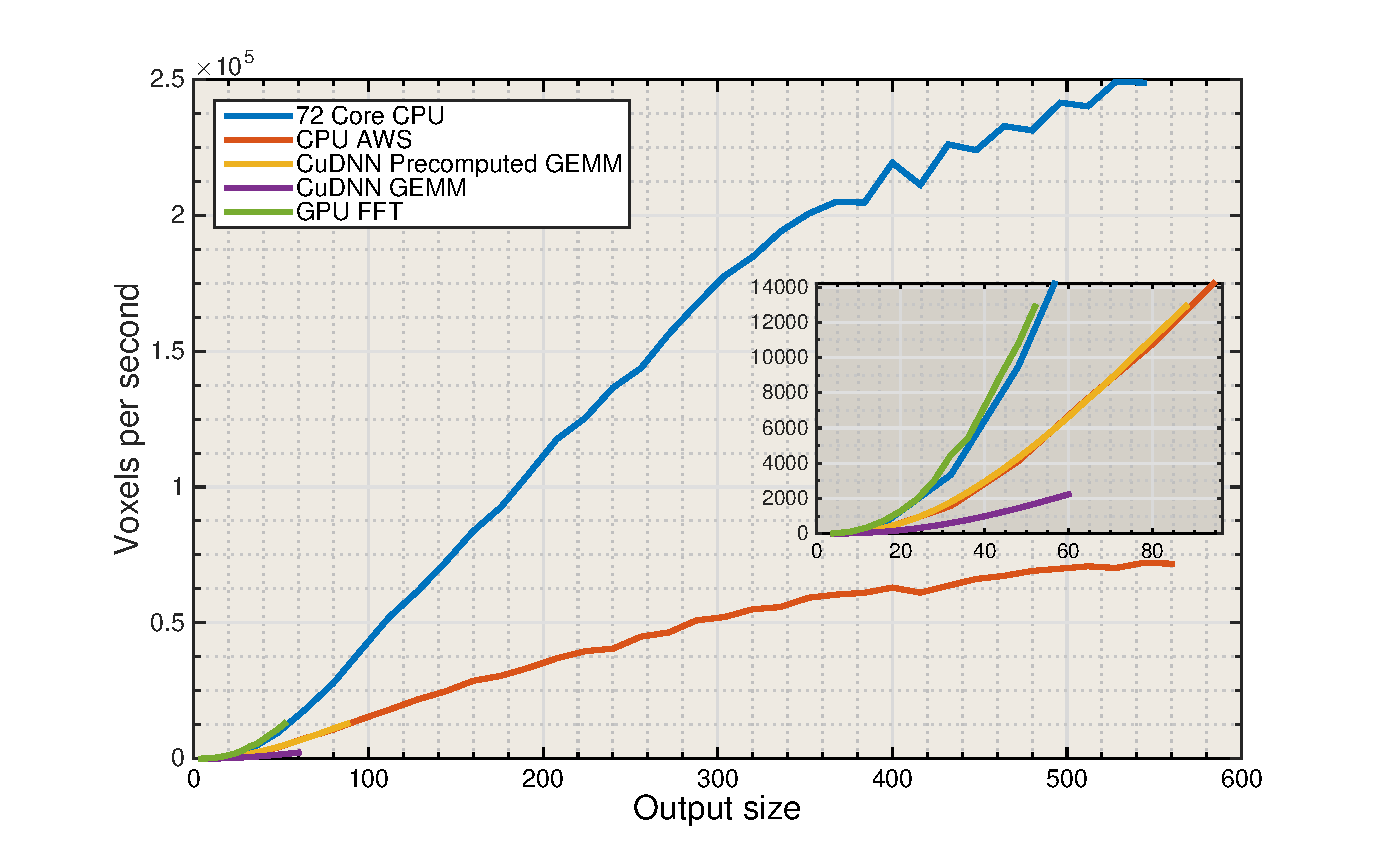
\includegraphics[width=0.44\textwidth]
    {fig/m96.eps}}
  \subfloat[]{\protect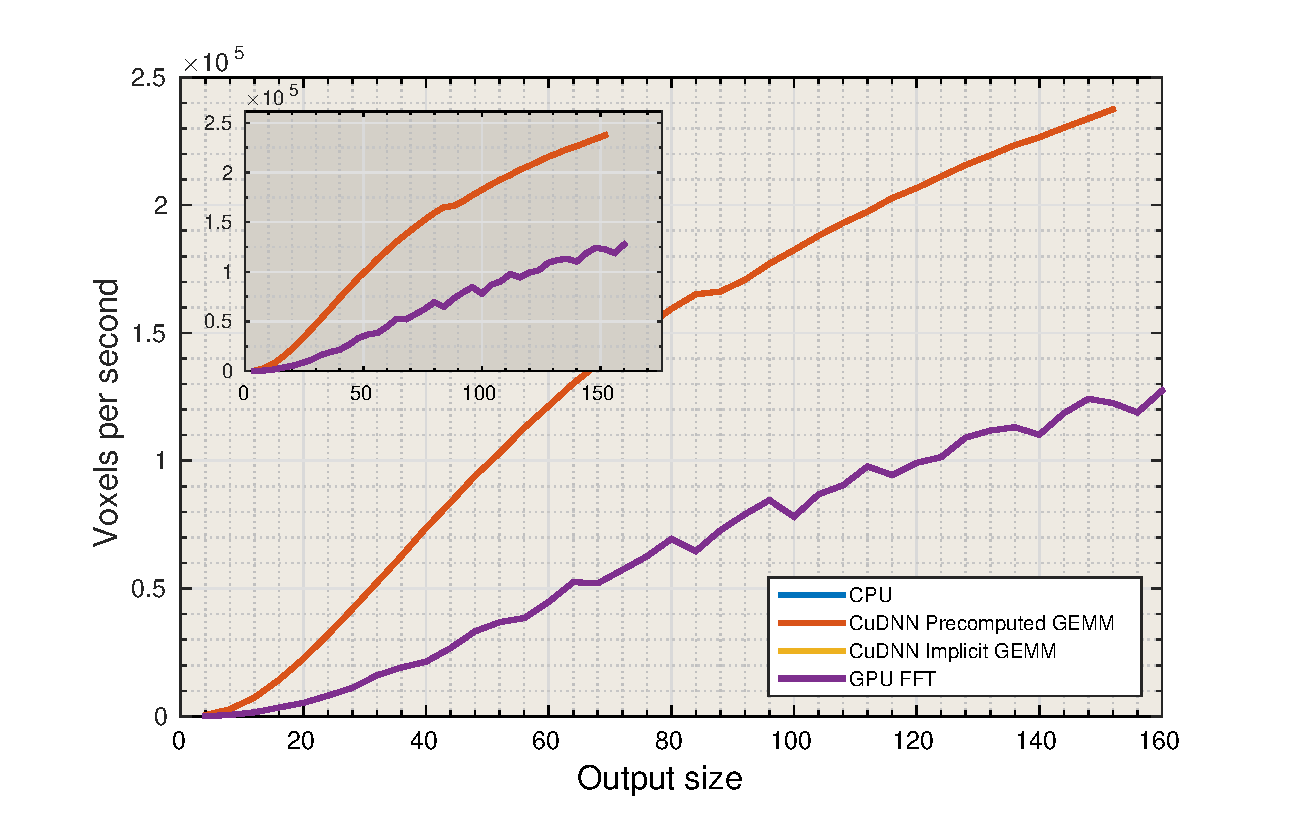
\includegraphics[width=0.44\textwidth]
    {fig/m56.eps}}
    \\
  \subfloat[]{\protect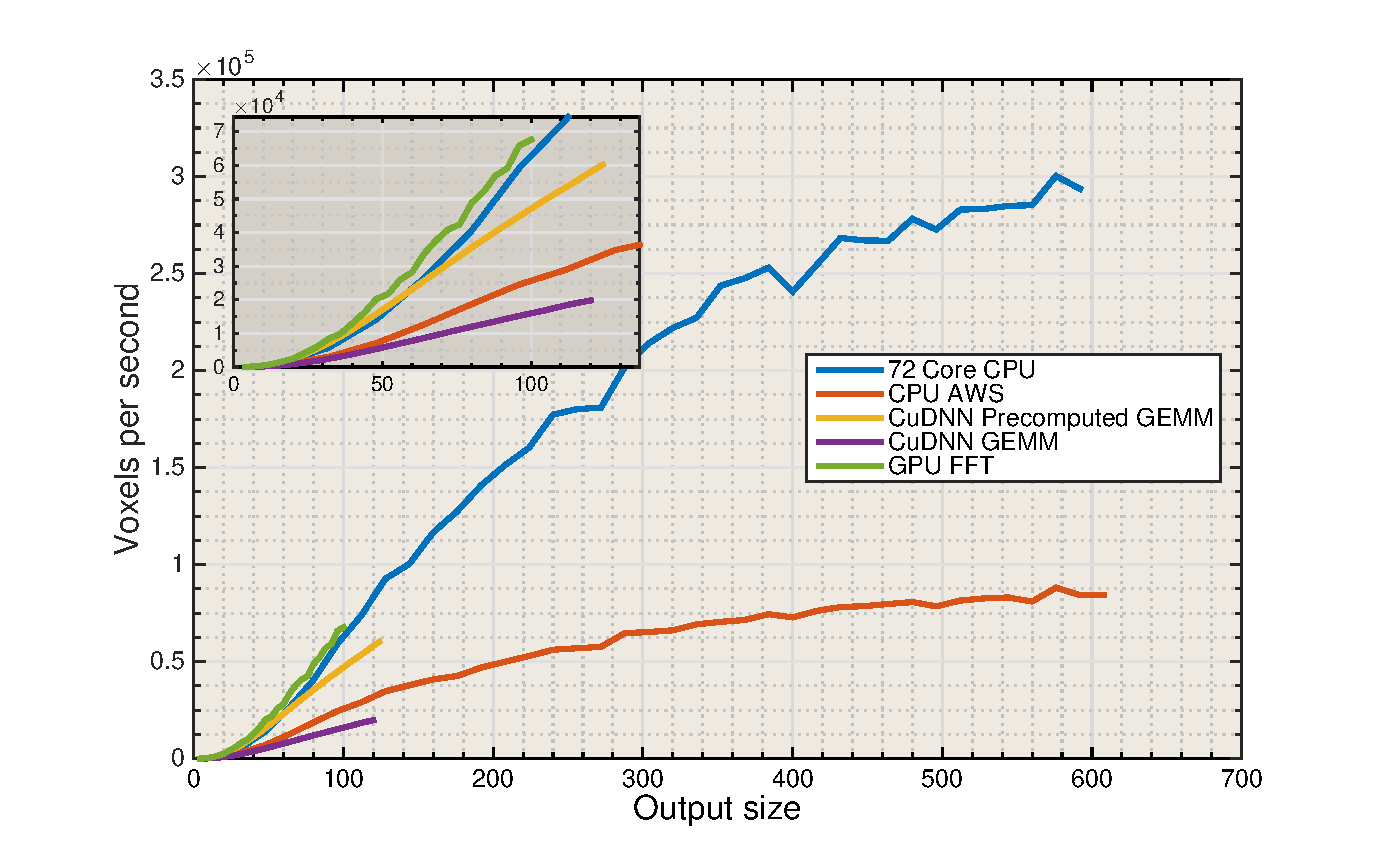
\includegraphics[width=0.44\textwidth]
    {fig/m76.eps}}
  \subfloat[]{\protect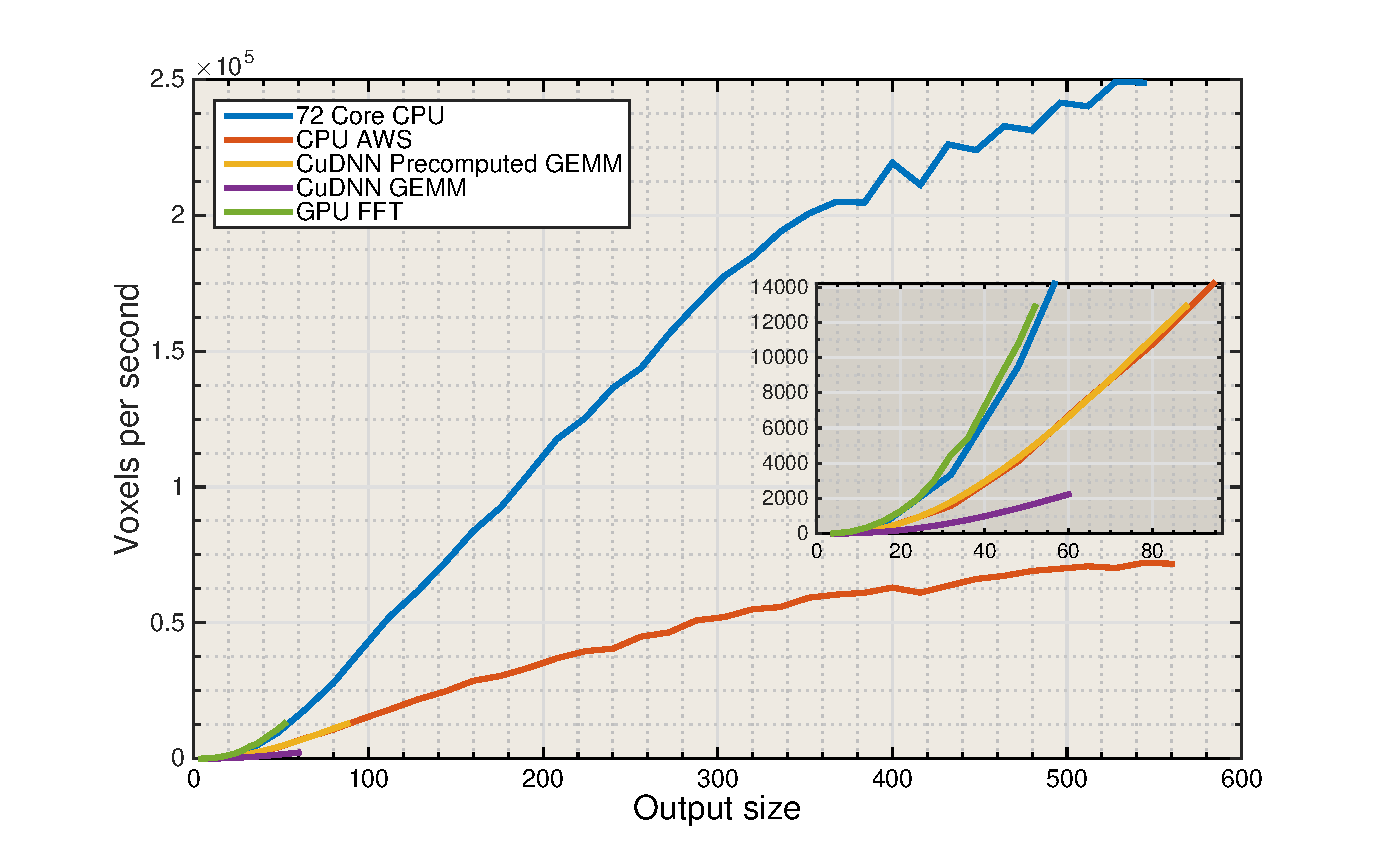
\includegraphics[width=0.44\textwidth]
    {fig/m96.eps}}

  \caption{Throughput vs output patch size for pooling networks
  }
  \label{fig:2dspeedups_threads}
\end{figure*}


%%%%%%%%%%%%%%%%%%%%%%%%%%%%%%%%%%%%%%%%%%%%%%%%%%%%%%%%%%%%%%%%%%%%%%%
%%%%%%%%%%%%%%%%%%%%%%%%%%%%%%%%%%%%%%%%%%%%%%%%%%%%%%%%%%%%%%%%%%%%%%%
%%
%% REFERENCES
%%
%%%%%%%%%%%%%%%%%%%%%%%%%%%%%%%%%%%%%%%%%%%%%%%%%%%%%%%%%%%%%%%%%%%%%%%
%%%%%%%%%%%%%%%%%%%%%%%%%%%%%%%%%%%%%%%%%%%%%%%%%%%%%%%%%%%%%%%%%%%%%%%


{\small
\bibliographystyle{IEEEtran}
\bibliography{IEEEabrv,./ref/bib}
}

\end{document}

%% ZNN - A Fast and Furious Technique for Training ConvNets on
%% Multi-Core and Many-Core Shared Memory Machines

%% C = 5 (or 2.5) should be mentioned somewhere?
